\documentclass[a4paper,11pt]{article}
\usepackage[left=2.5cm, right=2.5cm, top=1.5cm, bottom=1.5cm]{geometry}
\usepackage{graphicx}
\usepackage{amssymb}
\usepackage{amsmath}
\usepackage{xcolor}
\usepackage{hyperref}

\hypersetup{ %color attributes of citation, link, etc.
    colorlinks=true,
    linkcolor=blue,
    filecolor=gray,
    urlcolor=blue,
    citecolor=blue,
}

\setlength{\parindent}{0pt}

\newcommand{\matlab}{\textsc{Matlab}} %very important and totally necessary addition
\newcommand{\parallelsum}{\mathbin{\!/\mkern-5mu/\!}}

\newcommand\Item[1][]{%
  \ifx\relax#1\relax  \item \else \item[#1] \fi
  \abovedisplayskip=0pt\abovedisplayshortskip=0pt~\vspace*{-\baselineskip}}

%'codify' text for snippets
\usepackage{xcolor}
\definecolor{codegray}{gray}{1}
\newcommand{\code}[1]{\colorbox{codegray}{\texttt{#1}}}


\graphicspath{ {./images/} }
           
\begin{document}
\title{\LARGE{\textbf{ECEN405 Lab 6 Report}}}
\author{Niels Clayton : 300437590}
\date{}
\maketitle
\hrule

\begin{figure}[h!]
    \centering
    \frame{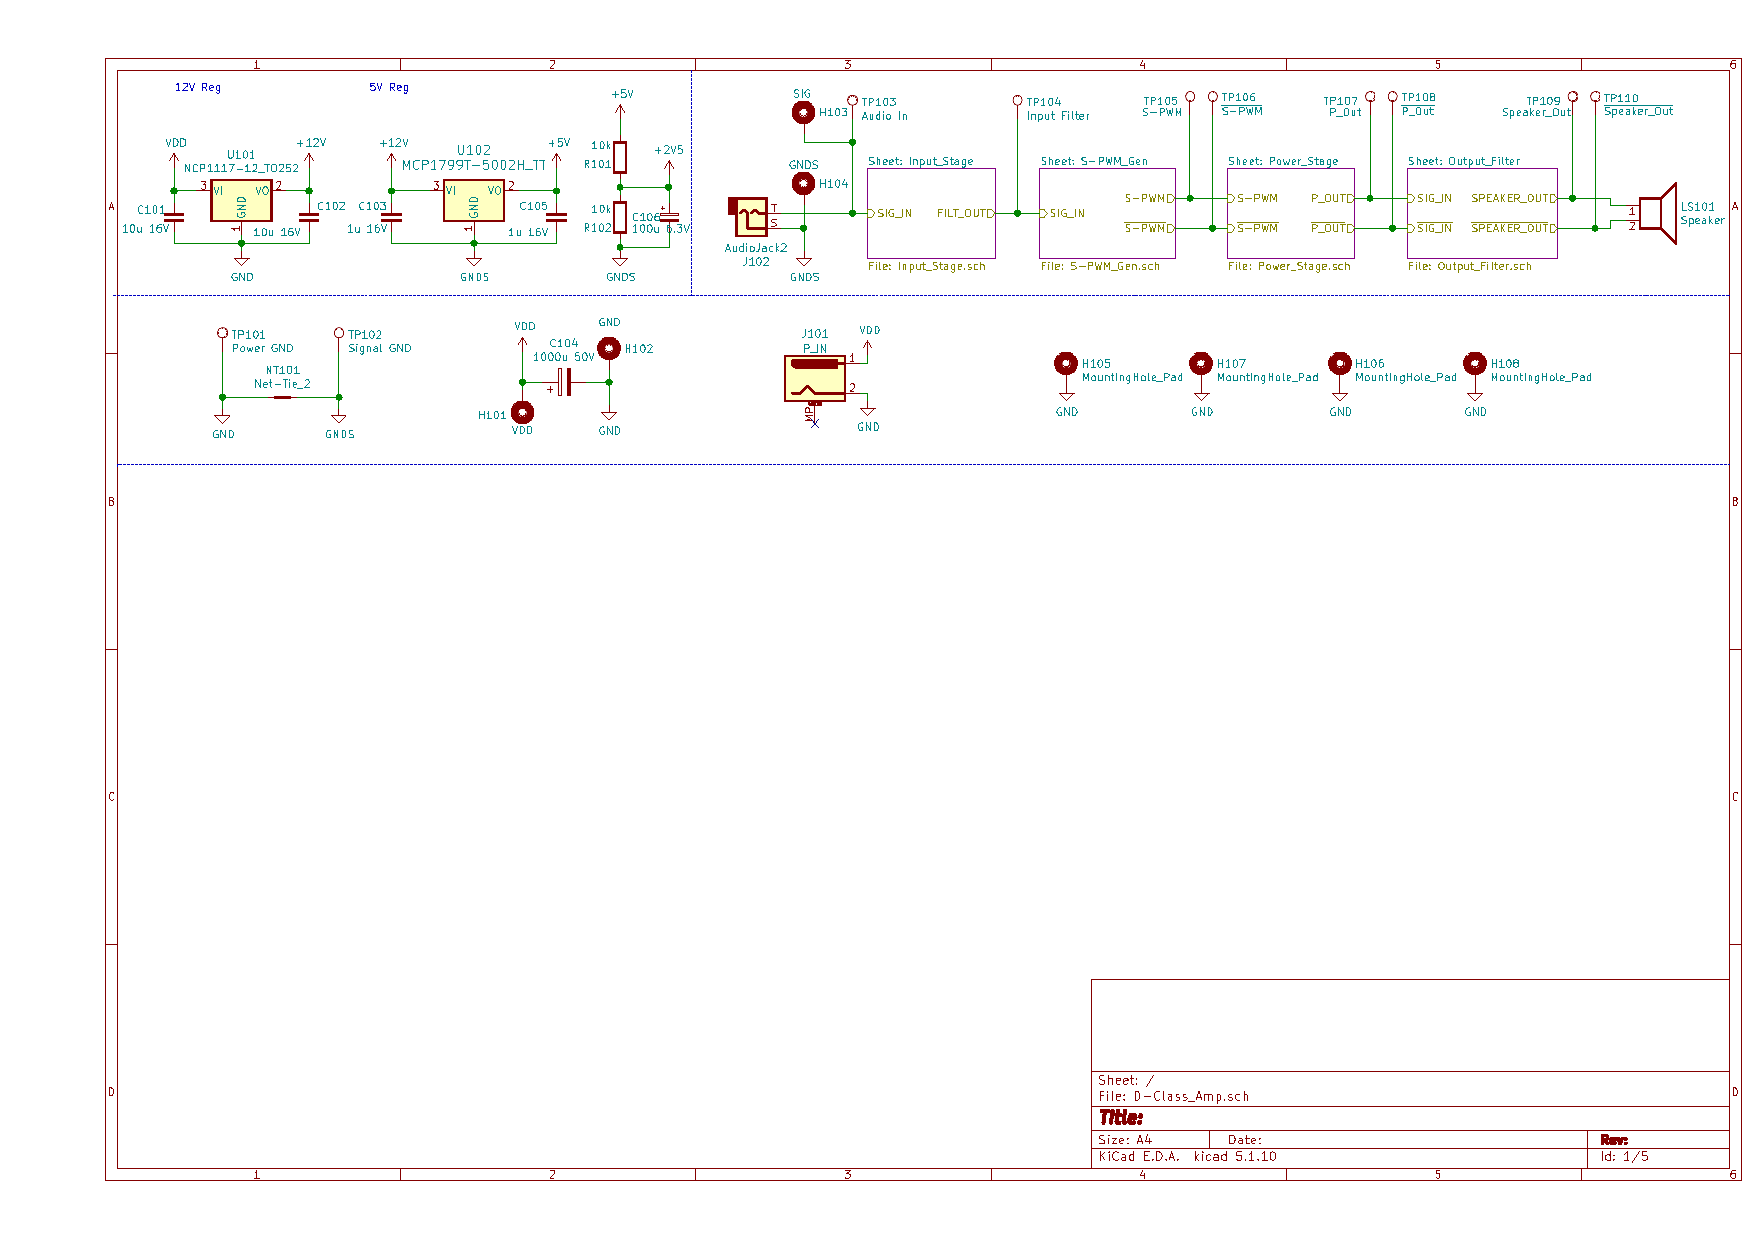
\includegraphics[page=1, trim={18mm 132mm 2mm 10mm},clip,width=0.85\textwidth]{pcb/schematic.pdf}}
    \caption{High level design schematic}
\end{figure}

\begin{figure}[h!]
    \centering
    \frame{\includegraphics[page=2, trim={25mm 70mm 90mm 60mm},clip,width=0.85\textwidth]{pcb/schematic.pdf}}
    \caption{Input filtering schematic}
\end{figure}

\begin{figure}[h!]
    \centering
    \frame{\includegraphics[page=3, trim={35mm 133.5mm 30mm 15mm},clip,width=0.85\textwidth]{pcb/schematic.pdf}}
    \caption{Sampling triangle wave \& SPWM generation schematic}
\end{figure}

\begin{figure}[h!]
    \centering
    \frame{\includegraphics[page=5, trim={85mm 149mm 5mm 12mm},clip,width=0.85\textwidth]{pcb/schematic.pdf}}
    \caption{Gate driver schematic}
\end{figure}

\begin{figure}[h!]
    \centering
    \frame{\includegraphics[page=4, trim={115mm 97mm 105mm 75mm},clip,width=0.6\textwidth]{pcb/schematic.pdf}}
    \caption{Output filter schematic}
\end{figure}


\end{document}